%!TEX ROOT=main.tex

\section{LoRa Module design}
As discussed in section \ref{section:module-architecture}, where the LoRa module was architected and its main parts were selected, the schematic and board layout were created. These outputs are included in image form as Appendix \ref{chapter:module01-files} along with more details and available at (https://github.com/manakjiri/lora-module-hw/releases/tag/v0.1)?.

The Open source KiCad Electronic Design Automation (EDA) software was used throughout the project to create these designs. 

\subsection{Schematic}
While the \ref{section:module-architecture} focused on the fundamental parts of the design, many details were left up to the later development stages, once the overall system implementation is more clear. This section will focus and expand on these parts of the design.

Of note is the selection of the main clock source for the MCU \ref{section:mcu}. In this case the only two options are to use a Crystal oscillator (XO) or an Temperature Compensated XO (TCXO). Application note AN5646 (STMicroelectronics) summarizes the main differences as
\begin{itemize}
    \item An XO is more efficient on power consumption, startup time, and BOM cost.
    \item A TCXO is more efficient on frequency accuracy and frequency variation over temperature changes. It also
    removes layout constraints.
\end{itemize}

This aspect was not considered carefully enough during the parts selection, the recommended NX2016SA series crystal oscillator was selected for the power savings and reduced cost. However, the selected programming framework embassy, and the library lora-rs in particular (expanded upon in Appendix \ref{chapter:rust}), only correctly supported the use of an TCXO, at the time of the prototype bring-up. This led to an ad-hoc modification \ref{fig:tcxo-bodge} of the module and the addition of the Abracon ATX-11-F series TCXO to fix this issue.

\begin{figure}
    \centering
    \subfloat[top view]{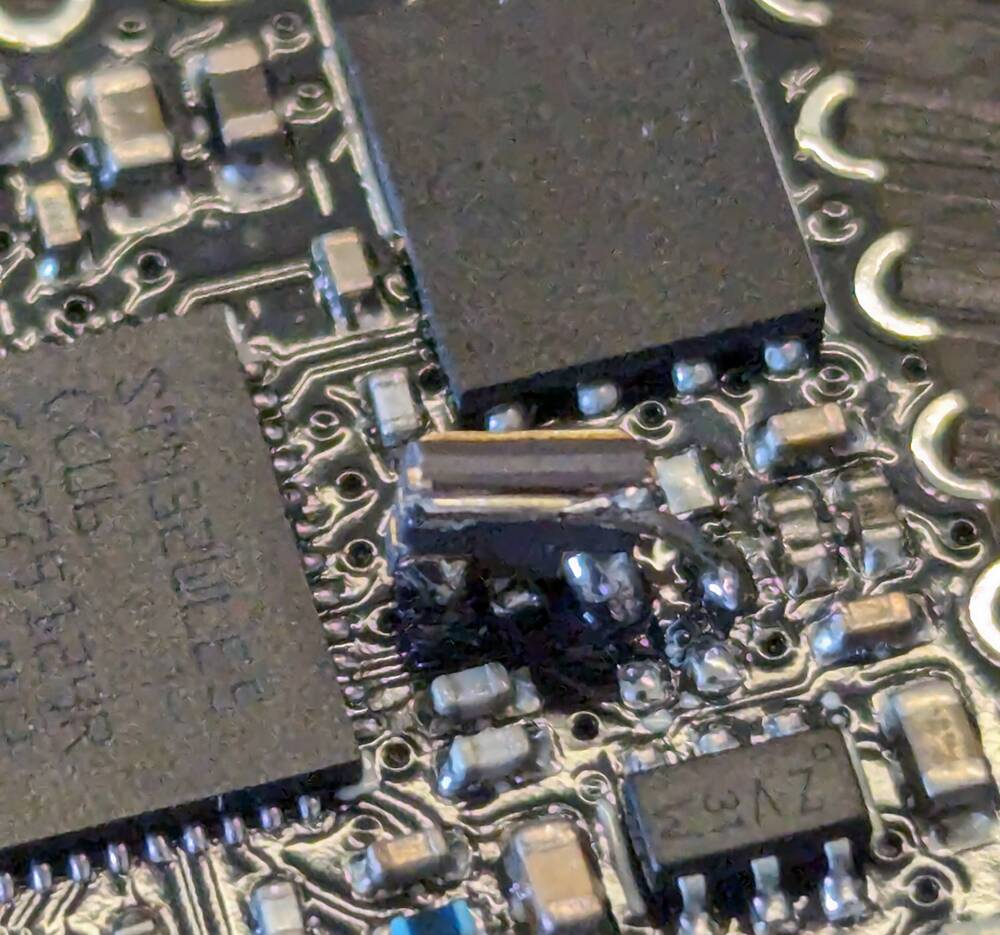
\includegraphics[width=.30\textwidth]{img/tcxo-bodge1.jpg}} \hfil
    \subfloat[side view]{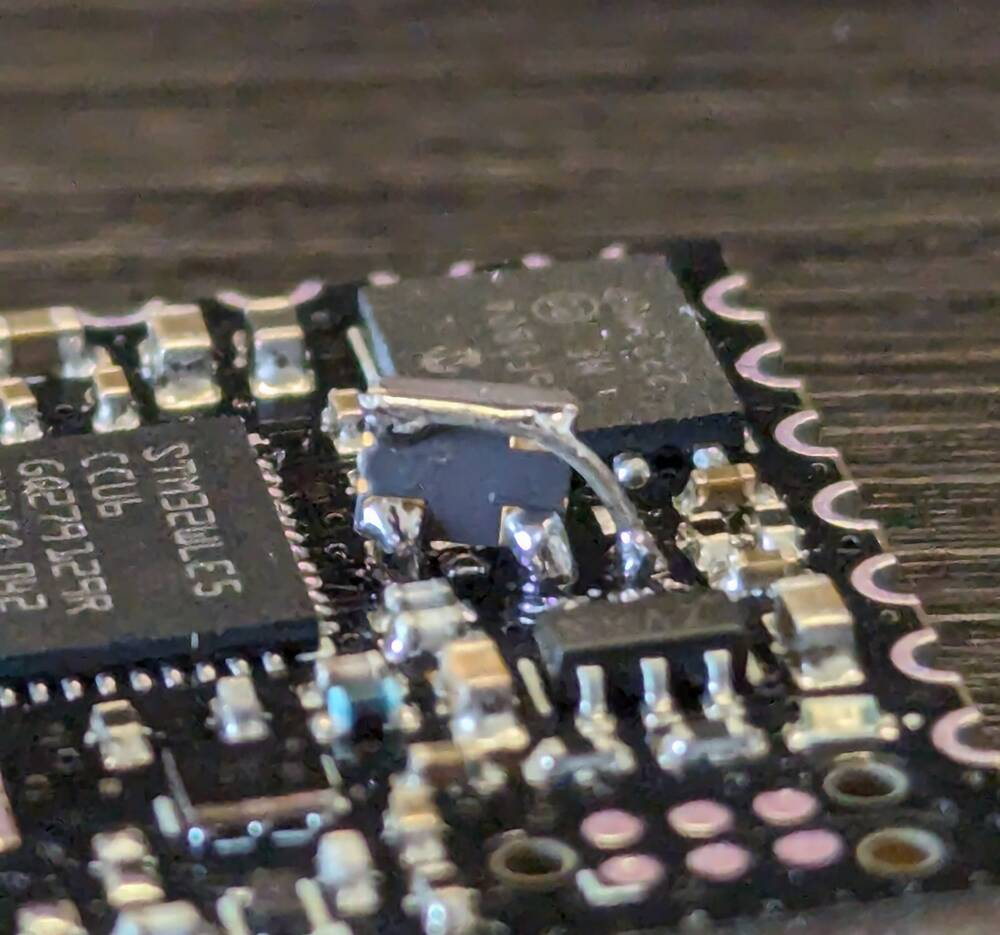
\includegraphics[width=.30\textwidth]{img/tcxo-bodge2.jpg}}
    \caption{\label{fig:tcxo-bodge}The ad-hoc TCXO modification on the LoRa module}
\end{figure}

All other aspects of the MCU integration were executed according to the application notes (cite) and the datasheet, while closely following the implementations of the reference design and the nucleo development kit. This includes the selection of decoupling capacitors, the SMPS circuitry and the reset handling.

Another consideration was the implementation of the switchable power rail VDD\_SW. This rail taps off the main power rail of the rest of the module, any disruption could cause a glitch or trigger the BOR protection circuitry. It is thus necessary to limit the inrush current caused by this rail's switch-on and subsequent charging of any local capacitances.

dopsat vypocty casu

\subsection{Board layout}
A 4 layer board stackup was proposed in Section \ref{section:mcu}, which indeed ended up being used in this design. Purpose of each layer is described in table \ref{table:board-layers} and clearly observable in the final renders \ref{board:v0.1}.

\begin{table}[H]
\begin{center}
\caption{\label{table:board-layers}Module board layer signal and power assignments}
    \begin{tabular}{|l|l|} \hline
    \textbf{Layer name}     & \textbf{Primary purpose} \\ \hline
    F. Front layer          & Components and local connections \\ \hline
    1. First inner layer    & Ground \\ \hline
    2. Second inner layer   & Power \\ \hline
    B. Back layer           & Signal and markings \\ \hline
    \end{tabular}
\end{center}
\end{table}

The board is only populated on the front side \ref{board:v0.1-components}, to allow its use as a solder-able module. Still, the final dimensions of the module are $20.32 \times 22.48~\mathrm{mm}$, which is better than the initial optimistic estimate given in \ref{section:antenna}.

To stay compatible with low-cost manufacturing options, conservative parameters were picked when it comes to minimal clearance, trace width and drill size. No density-increasing technologies, such as blind or buried vias, via-in-pad, micro-via, etc. were not employed either. 

These parameters are summarized in the following Table \ref{table:board-limits} and were enforced by the Design Rule Checker (DRC) throughout the project.

\begin{table}[H]
\begin{center}
\caption{\label{table:board-limits}Board layout physical limits}
    \begin{tabular}{|l|l|} \hline
    \textbf{Parameter}          & \textbf{Dimension} \\ \hline
    Minimum trace clearance & $0.15~\mathrm{mm}$ \\ \hline
    Minimum trace width & $0.15~\mathrm{mm}$ \\ \hline
    Minimum via width & $0.3~\mathrm{mm}$ \\ \hline
    Hole to trace clearance & $0.3~\mathrm{mm}$ \\ \hline
    Hole to hole clearance & $0.5~\mathrm{mm}$ \\ \hline
    Board edge to trace clearance & $0.15~\mathrm{mm}$ \\ \hline
    \end{tabular}
\end{center}
\end{table}

Being only 4 layers, the traces needed to be routed in densely and well thought-out manner, attempting to minimize the number of relatively large vias required. For this reason, the module's external connection signal assignments were decided only near the end of the design stage conforming mostly to the existing pin locations on the MCU itself. The final pad assignments are included in Table \ref{table:module-pin-legend}.

\subsection{Final module specification}
\begin{figure}
    \includesvg[width=.75\textwidth]{img/module-v0.1.drawio.svg}
    \caption{\label{fig:module-v0.1}Image of the manufactured and fully assembled module with overlay highlighting its functional parts}
\end{figure}

\begin{table}[H]
\begin{center}
\caption{\label{table:module-specification}Final module specification}
    \begin{tabular}{|l|l|} \hline
    Supply voltage range                    & $2.3\text{--}3.5~\mathrm{V}$\\ \hline
    Maximum supply current (excluding EXT)  & $65~\mathrm{mA}$\\ \hline
    Standby supply current                  & $?~\mathrm{uA}$\\ \hline
    Operating temperature range             & $-40\text{--}85~\mathrm{^\circ C}$\\ \hline
    Output RF power                         & $15~\mathrm{dB}$\\ \hline
    Operating band                          & $868~\mathrm{MHz}$\\ \hline
    RF connector                            & U.FL \\ \hline
    Module connection type                  & Castellated hole (0.1 inch pitch) \\ \hline
    Supported interfaces                    & UART, SPI, I2C \\ \hline
    Programming interface                   & ARM Serial Wire Debug \\ \hline
    \end{tabular}
\end{center}
\end{table}

\begin{table}[H]
\begin{center}
\caption{\label{table:module-pin-legend}Module pin legend including feature summary.}
    \begin{tabular}{|l|l|l|l|l|l|l|l|l|} \hline
    \textbf{IO} & \textbf{Pin} & \textbf{TIM\footnote{Refer to each column following ``Pin'' (excluding ``Other'') as [Column header][Column-row contents], such as ``SPI1\_MOSI'' and so on. Some features were omitted for clarity, for complete list refer to the MCU manufacturer's documentation}} & \textbf{ADC} & \textbf{I2C} & \textbf{SPI} & \textbf{UART} & \textbf{Other}\\ \hline
    1  & PA7  & 17\_1, 1\_1N    &     & 3\_SCL & 1\_MOSI &             & CMP2\_OUT          \\ \hline
    2  & PA6  & 16\_1          &     &       & 1\_MISO &             &                    \\ \hline
    3  & PA4  & L1,2\_OUT      &     &       &        &             & RTC\_OUT2           \\ \hline
    4  & PA2  & 2\_3           &     &       &        & 2\_TX      & CMP2\_OUT           \\ \hline
    5  & PA1  & L3\_OUT, 2\_2   &     &       & 1\_SCK  &             &                    \\ \hline
    6  & PA0  & 2\_1           &     &       &        &             & WKUP1   \\ \hline
    7  & PB8  & 16\_1, 1\_2N    &     & 1\_SCL &        &             &                    \\ \hline
    8  & PB7  & L1\_IN2, 17\_1N &     & 1\_SDA &        & 1\_RX        &                    \\ \hline
    9  & PB6  &               &     & 1\_SCL &        & 1\_TX        &                    \\ \hline
    10 & PB5  & L1\_IN1        &     &       & 1\_MOSI &             & CMP2\_OUT          \\ \hline
    11 & PB4  &               & 3   & 3\_SDA & 1\_MISO &             & CMP1,2\_INP        \\ \hline
    12 & PA11 & 1\_4           & 7   & 2\_SDA & 1\_MISO &             & CMP1,2\_INM        \\ \hline
    13 & PB3  & 2\_CH2         & 2   &       & 1\_SCK  &             & SWO, WKUP3 \\ \hline
    14 & PA13 &               & 9   &       &        &             & SWDIO            \\ \hline
    15 & PA14 & L1\_OUT        & 10  &       &        &             & SWCLK                   \\ \hline
    16 & PH3  &               &     &       &        &             & BOOT0                   \\ \hline
    \end{tabular}
\end{center}
\end{table}

\section{Soil moisture sensor design}

\section{Over The Air update implementation}
It is the responsibility of the update process to securely and reliably transfer the binary image of the firmware from the host computer through the Gateway to the designated Node (sensor) of the network. This task is complicated by the limited resources available on embedded devices and the slow and sometimes unreliable nature of the wireless connection in general.

\subsection{Data fragmentation}
The binary needs to be fragmented in order to be transmitted piece by piece. To guarantee the assembly of these fragments on the Node, an acknowledge mechanism must be present along with a way to detect errors in the transferred data. While the LoRa physical layer provides forward error correction and also up to a 16 bit CRC checksum, the error rate is from experience still too high to be practical. To tackle this, a custom 32 bit CRC was used to protect each fragment together with a SHA256 hash of the whole assembled binary, which is calculated as the last step in the update process.

\begin{figure}[p]
    \includesvg[width=0.9\textwidth]{fig/ota-algo.drawio.svg}
    \caption{\label{fig:ota-algo}Simplified flowchart depicting the Over The Air update communication process between the Gateway and the Node}
\end{figure}

Figure \ref{fig:ota-algo} provides a basic overview of the OTA update process. The communication with the host is left out for brevity, but mostly mirrors the operations that happen on the Gateway. Names in the cells correspond to packet types defined in the \href{https://github.com/manakjiri/lora-module-fw/blob/main/module-runtime/src/ota/common.rs}{module-runtime/src/ota/common.rs} file as \lstinline|enum OtaPacket|. Packets are serialized and deserialized using the postcard Rust package.

\subsection{ACK mechanism}
The Automatic Repeat Request (ARQ) mechanism is inspired by Selective Repeat ARQ. The receiver is able to accept frames that are out of order and selectively requests missing or corrupted blocks, but the acknowledge (ACK) packet contains up to 32 indexes of blocks that were successfully received. 

Likewise, the transmitter does not expect to receive ACK packets consistently and continues to transmit in order for up to 16 unACKed frames. The receiver is thus able to relax the rate of ACK packets to reduce the air time usage. Since the transmitter is not attempting to use the maximum available channel capacity, it transmits about one packet per second, it does not need the immediate response to measure latency.

\section{Range test}
In order to determine the real-world performance, a range test was conducted. Primary points of interest are
\begin{itemize}
    \item maximum practically usable range of the solution and connection quality deterioration as the distance and occlusion increases,
    \item performance of the designed module compared with the Nucleo development board as reference,
    \item the effect of proximity of the antenna to the ground and
    \item the effect of the spreading factor (SF) modulation parameter.
\end{itemize}

All testing so far was done in home environment with Nodes in close proximity and no major packet loss could be observed. Given the relatively low experience in RF design however, it is expected the module will perform worse than the Nucleo board.

With increasing spreading factor, the symbol time increases and the link budget goes with it, as can be seen in Table \ref{table:semtech-sf}. But longer symbol time relies on more stable and precise frequency reference. 

\begin{figure}[H]
    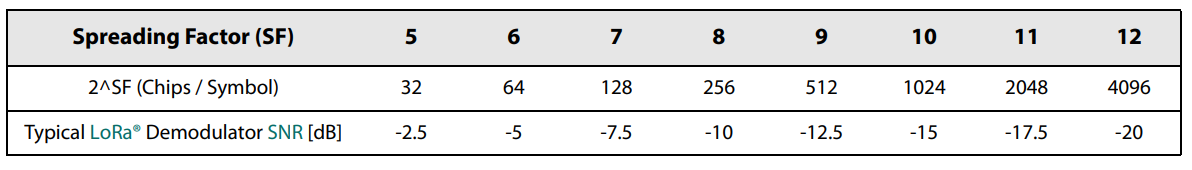
\includegraphics[width=\textwidth]{fig/semtech-sf-table.png}
    \caption{\label{table:semtech-sf}Range of Spreading Factors (SF)}
\end{figure}

Bandwidth variation exhibits similar traits, but to stay within the legal limits of the EU868 band, it is necessary to stay within $125\text{--}500~\mathrm{kHz}$. This is the reason for selecting SF as the variable, while keeping the Bandwidth and the coding rate (CR) constant. CR also has a very predictable effect on the connection quality.

\subsection{Hypothesis}
It is expected the proximity to the ground will have high impact on the usable range of the sensor, meaning Nodes mounted with their antenna closer to the ground should perform worse. Higher SF should yield longer range. We are not expecting to surpass distance of $1~\mathrm{km}$.

\subsection{Prerequisite}
The maximum achievable SF needed to be determined. This was done experimentally, starting with SF5 and incrementing util it was no longer possible to transfer data. This test was conducted using Nucleo acting as the initiator of connection with the LoRa module. Devices were situated on a desk about 1.5 meters apart with their antennae positioned orthogonally in respect to each other to avoid overwhelming the receiver. All other parameters are identical to those used in the latter experiment.

The connection was stable at SF11, but at SF12 the LoRa module stopped responding, thus the experiment was done at SF5 and SF11, which corresponds to a theoretical delta of $15~\mathrm{dB}$.

\subsection{Methodology}
All LoRa modulation and packet parameters were set in firmware (commit \href{https://github.com/manakjiri/lora-module-fw/tree/76acdcd7b31f259c88f1808ed79886dc26295b4e}{76acdcd}) identically for all devices used, a summary is provided in Table \ref{table:range-test-parameters}. 

\begin{table}[H]
\begin{center}
\caption{\label{table:range-test-parameters}LoRa parameters for range testing}
    \begin{tabular}{|l|l|} \hline
    Frequency             & $869.525~\mathrm{MHz}$\\ \hline
    RF power output       & $15~\mathrm{dB}$\\ \hline
    Bandwidth             & $250~\mathrm{kHz}$\\ \hline
    Coding rate           & $4:8$ (2x overhead) \\ \hline
    Bandwidth             & $250~\mathrm{kHz}$\\ \hline
    Preamble length       & $32~\mathrm{b}$\\ \hline
    Implicit header       & No\\ \hline
    LoRa CRC              & No\\ \hline
    Inverted IQ           & No\\ \hline
    Transmit boost        & No\\ \hline
    Receive boost         & No\\ \hline
    \end{tabular}
\end{center}
\end{table}

LoRa modules used the MOLEX 105262-0003 antenna and Nucleo boards used their stock antenna, all were close to vertical orientation. A pole with two LoRa modules and one Nucleo (see Figure \ref{fig:range-nodes}) was constructed to act as the stationary set of Nodes to test against. Another Nucleo board was attached to a car (see Figure \ref{fig:range-gateway}) to act as the Gateway, see Table \ref{table:range-test-devices} for more details.

\begin{table}[H]
\begin{center}
\caption{\label{table:range-test-devices}Devices used for range testing}
    \begin{tabular}{|l|l|l|} \hline
    \textbf{Device} & \textbf{Height\footnote{Measured distance from the root of the antenna to ground level} [m]} & \textbf{Address}\footnote{Data presented will use these addresses to distinguish between the different Nodes used in the experiment} \\ \hline
    Nucleo (Gateway) & 1.65 & 1 \\ \hline
    LoRa module (Node) & 0.19 & 2 \\ \hline
    Nucleo (Node) & 0.55 & 4 \\ \hline
    LoRa module (Node) & 0.82 & 3 \\ \hline
    \end{tabular}
\end{center}
\end{table}

\begin{figure}[p]
    \centering
    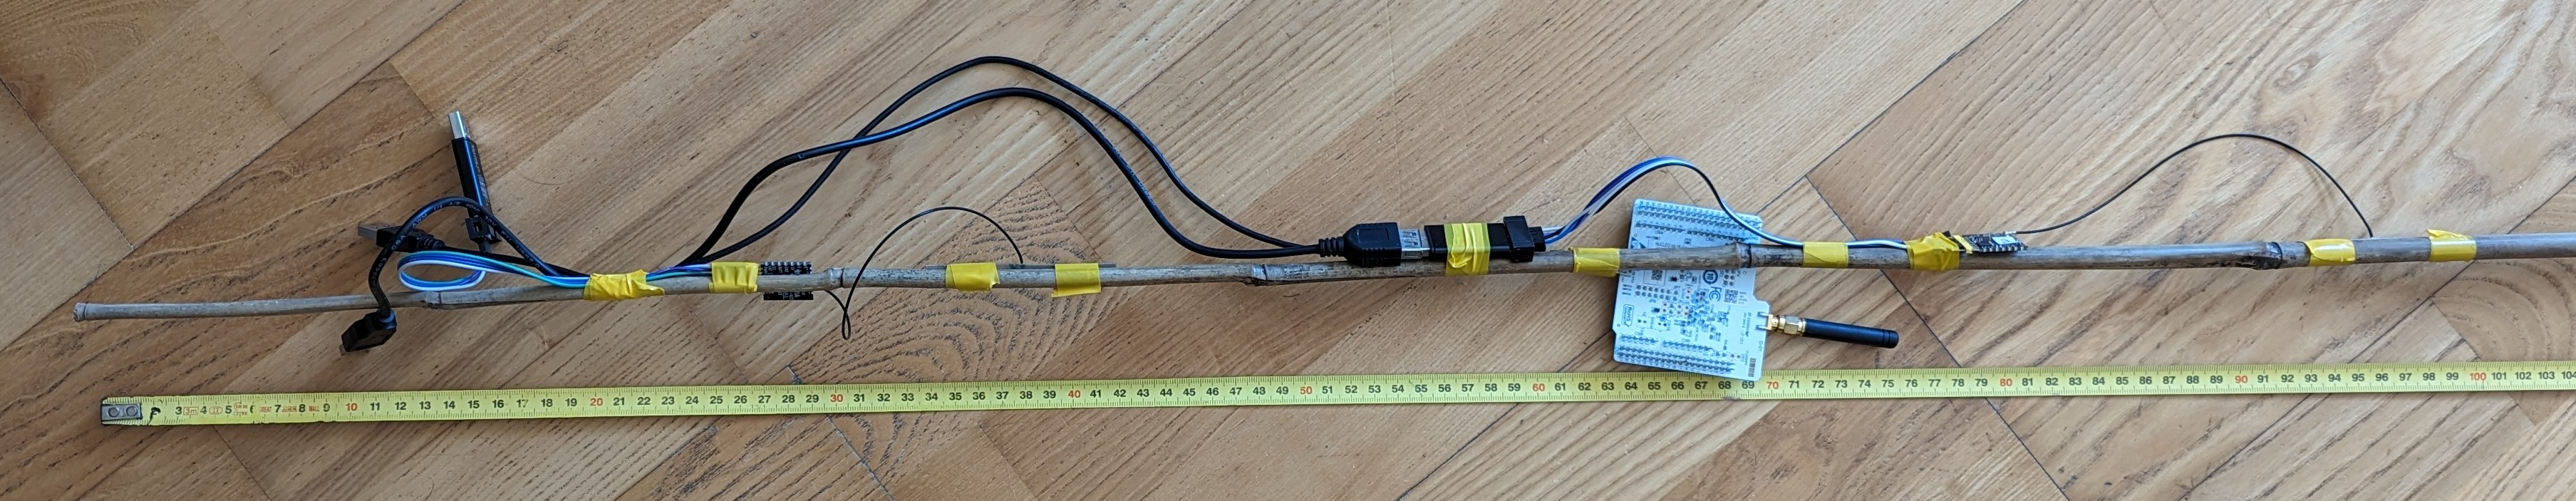
\includegraphics[width=.9\textwidth]{img/lora-pole.jpg}\vspace{1em}
    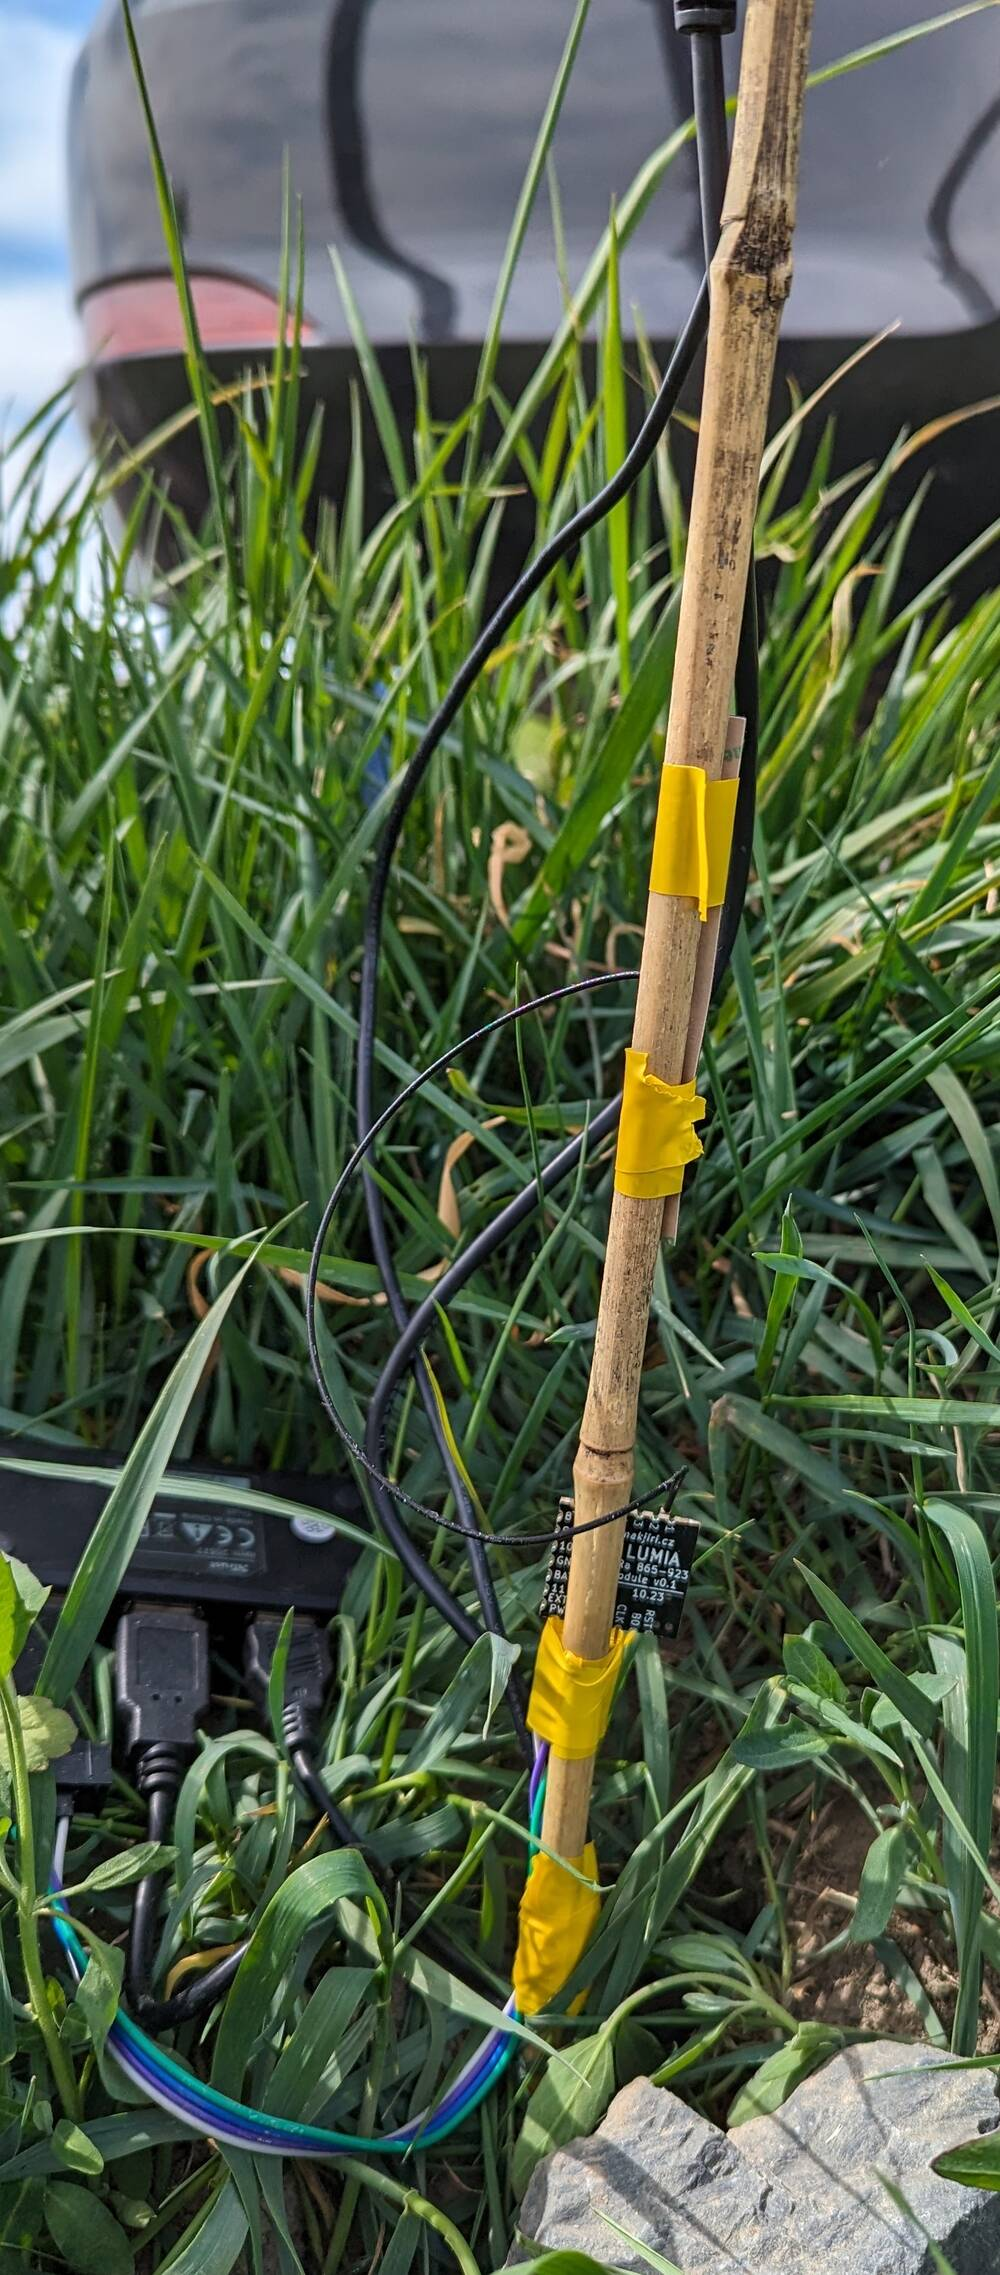
\includegraphics[width=.25\textwidth]{img/range-pole-base.jpg}\hfil
    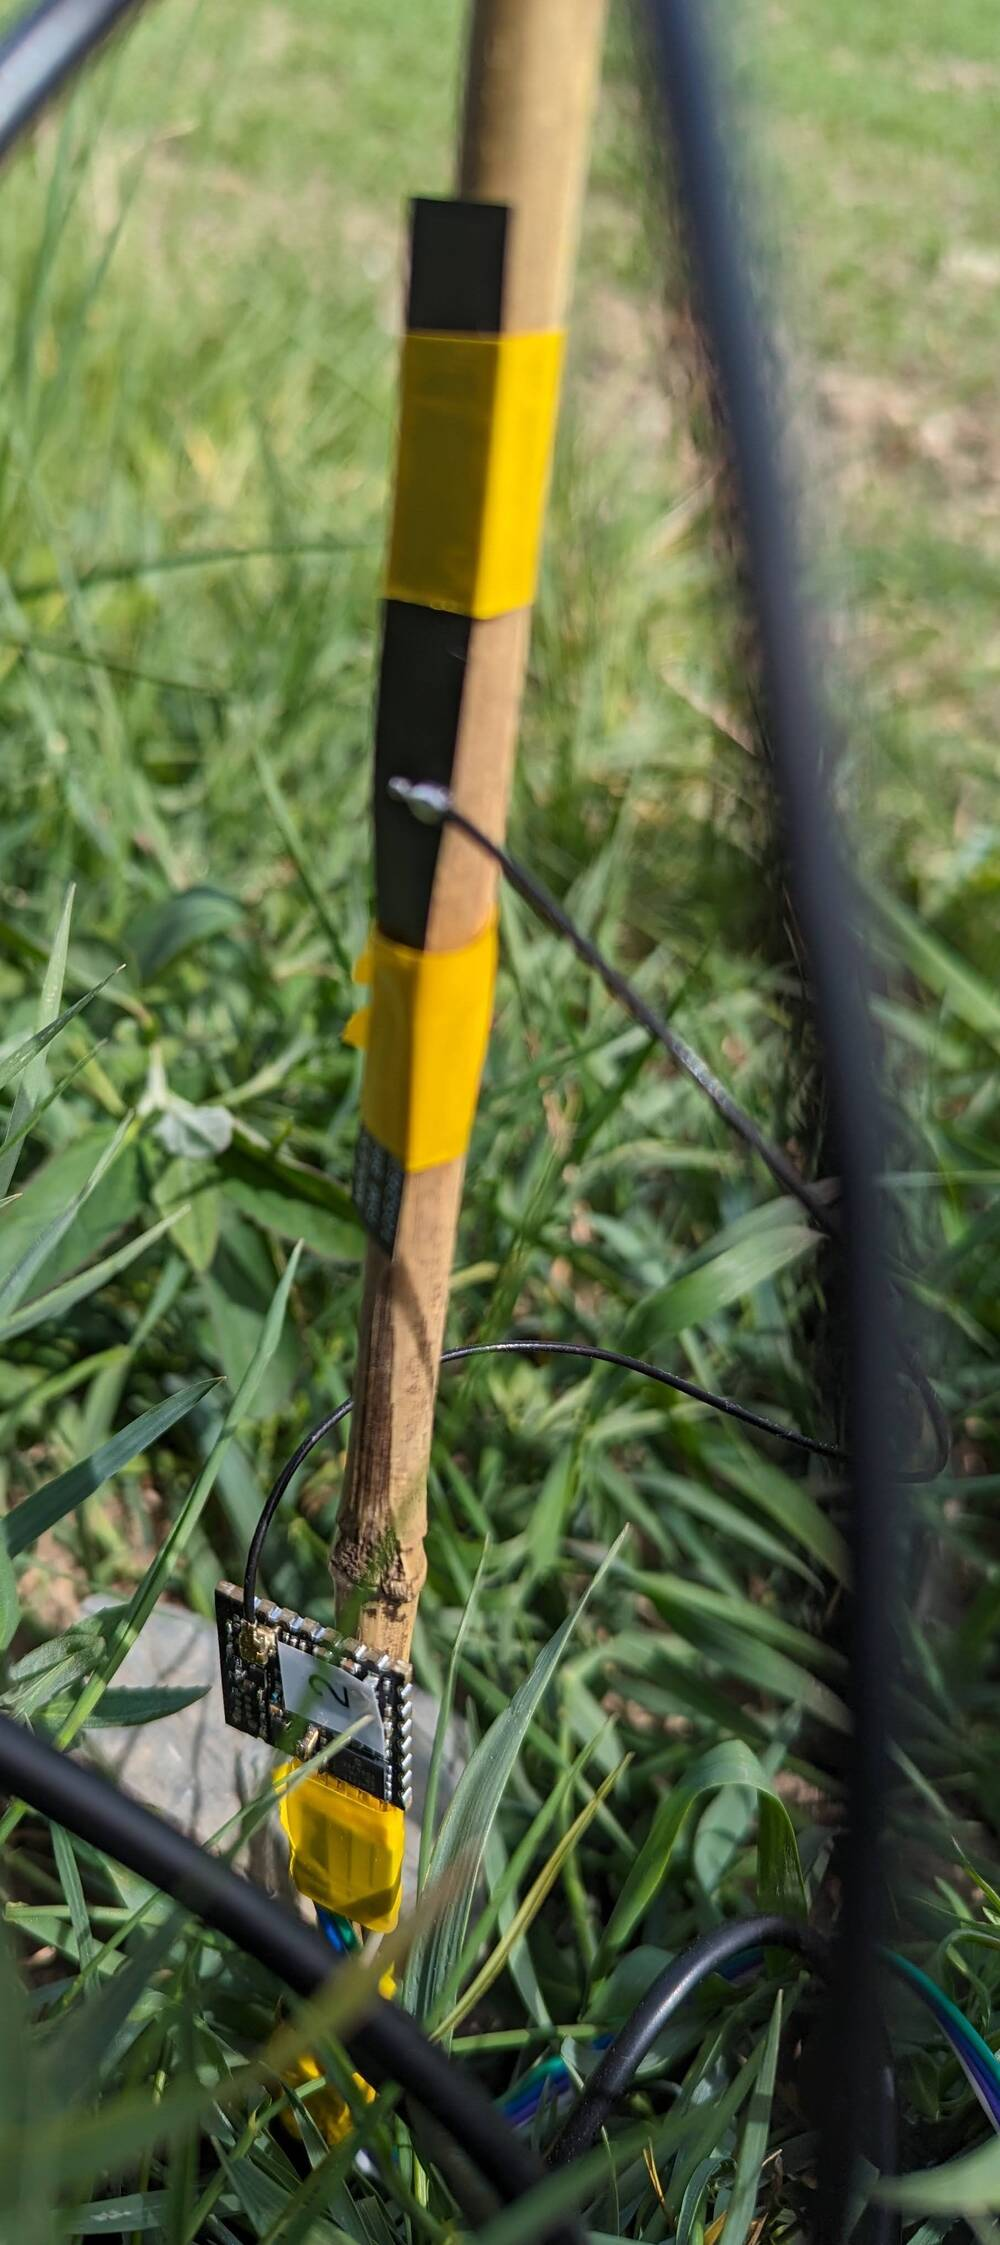
\includegraphics[width=.25\textwidth]{img/range-pole-bottom.jpg}\hfil
    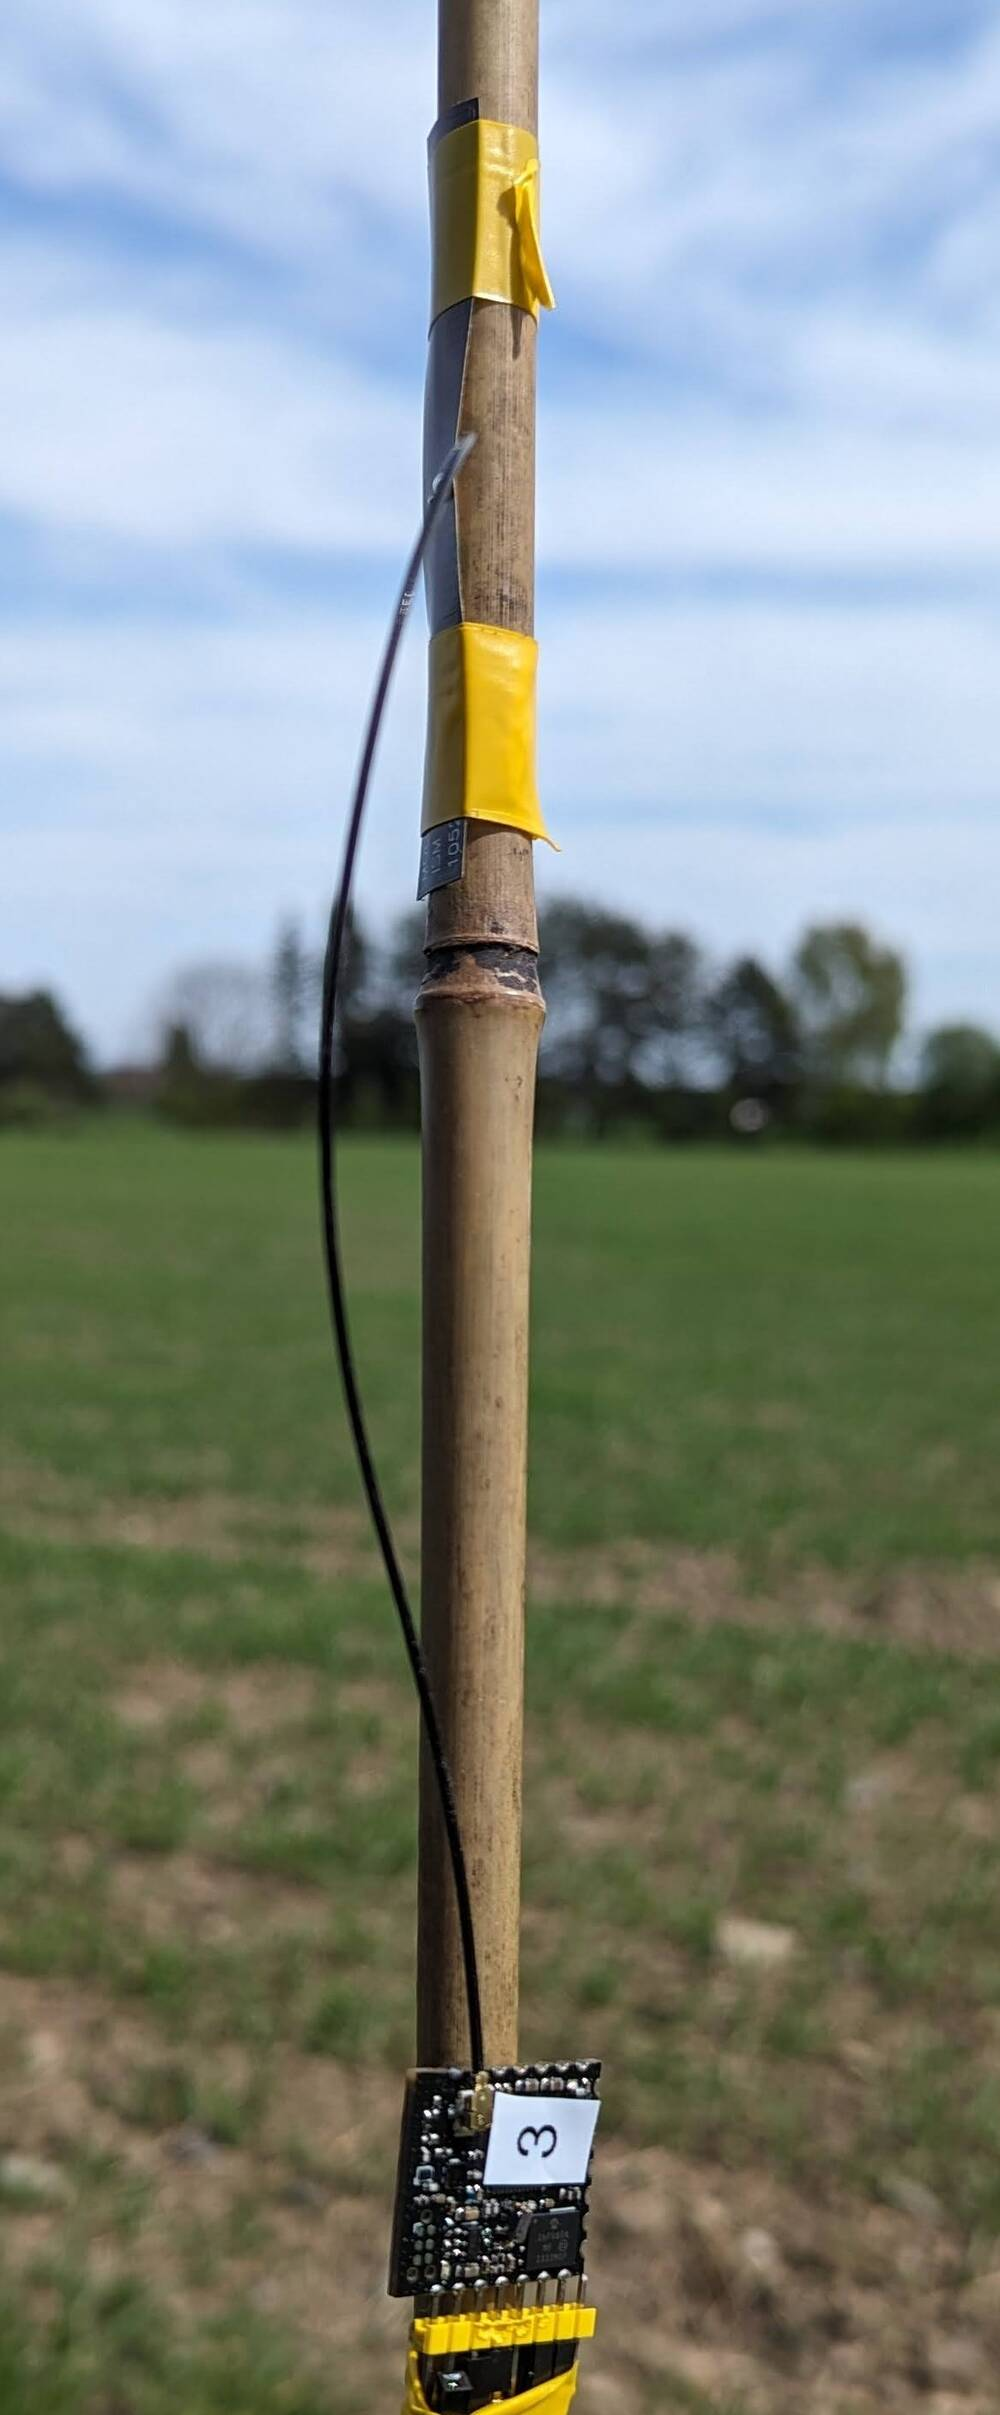
\includegraphics[width=.24\textwidth]{img/range-pole-top.jpg}
    \caption{\label{fig:range-nodes}Close-up of the pole with Nodes attached for range testing}
\end{figure}

\begin{figure}[p]
    \centering
    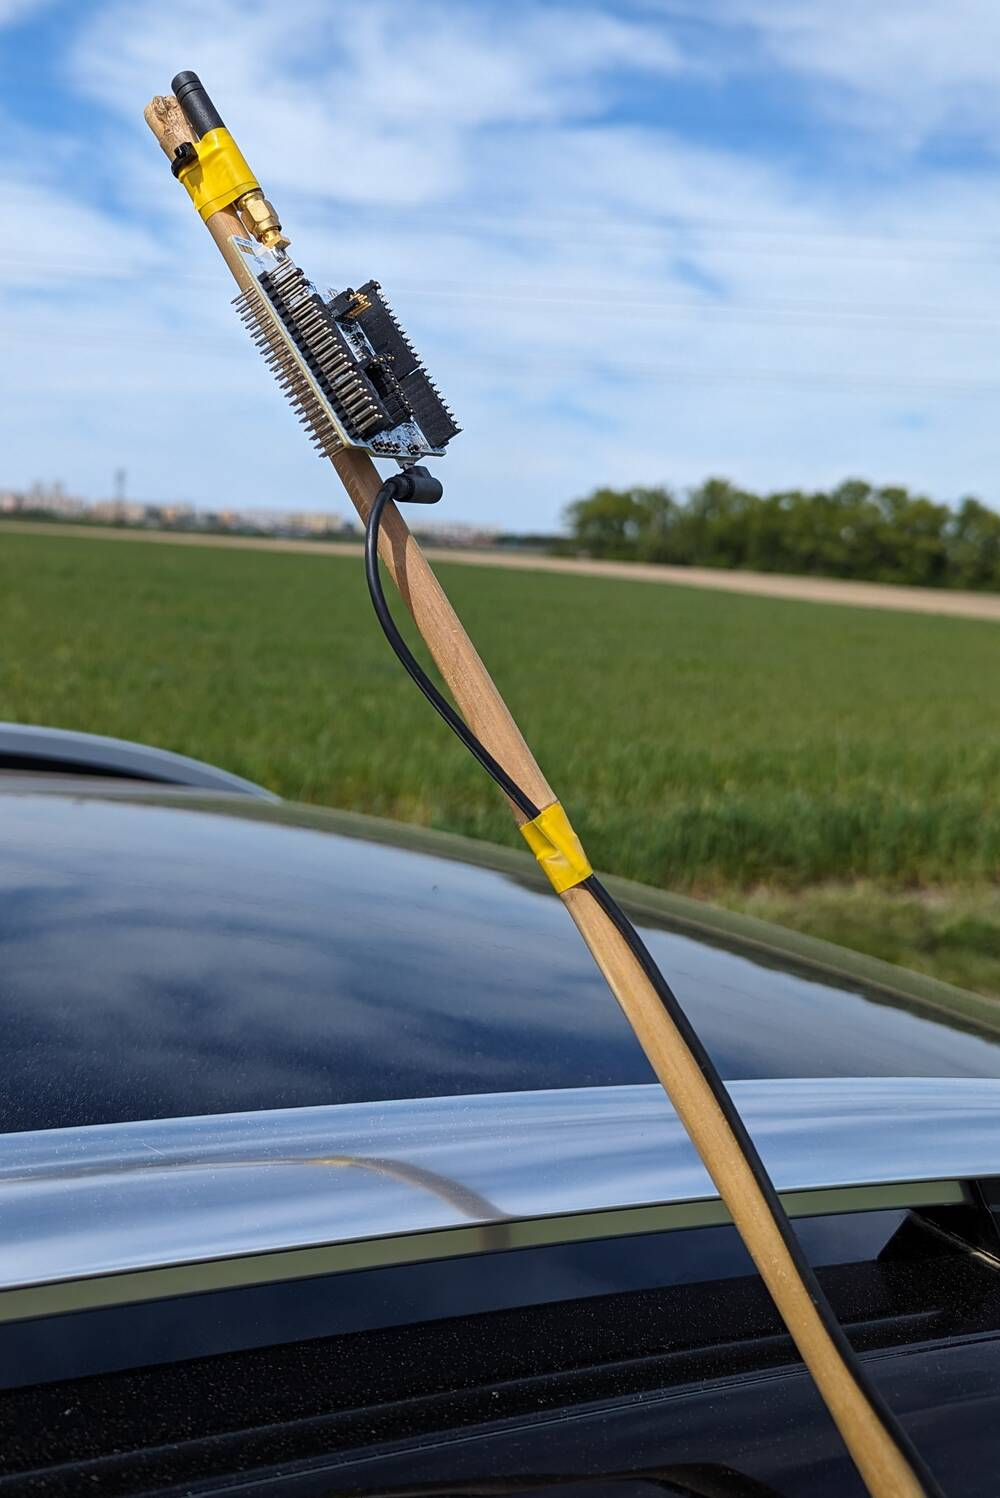
\includegraphics[width=.35\textwidth]{img/range-gateway1.jpg}\hfil
    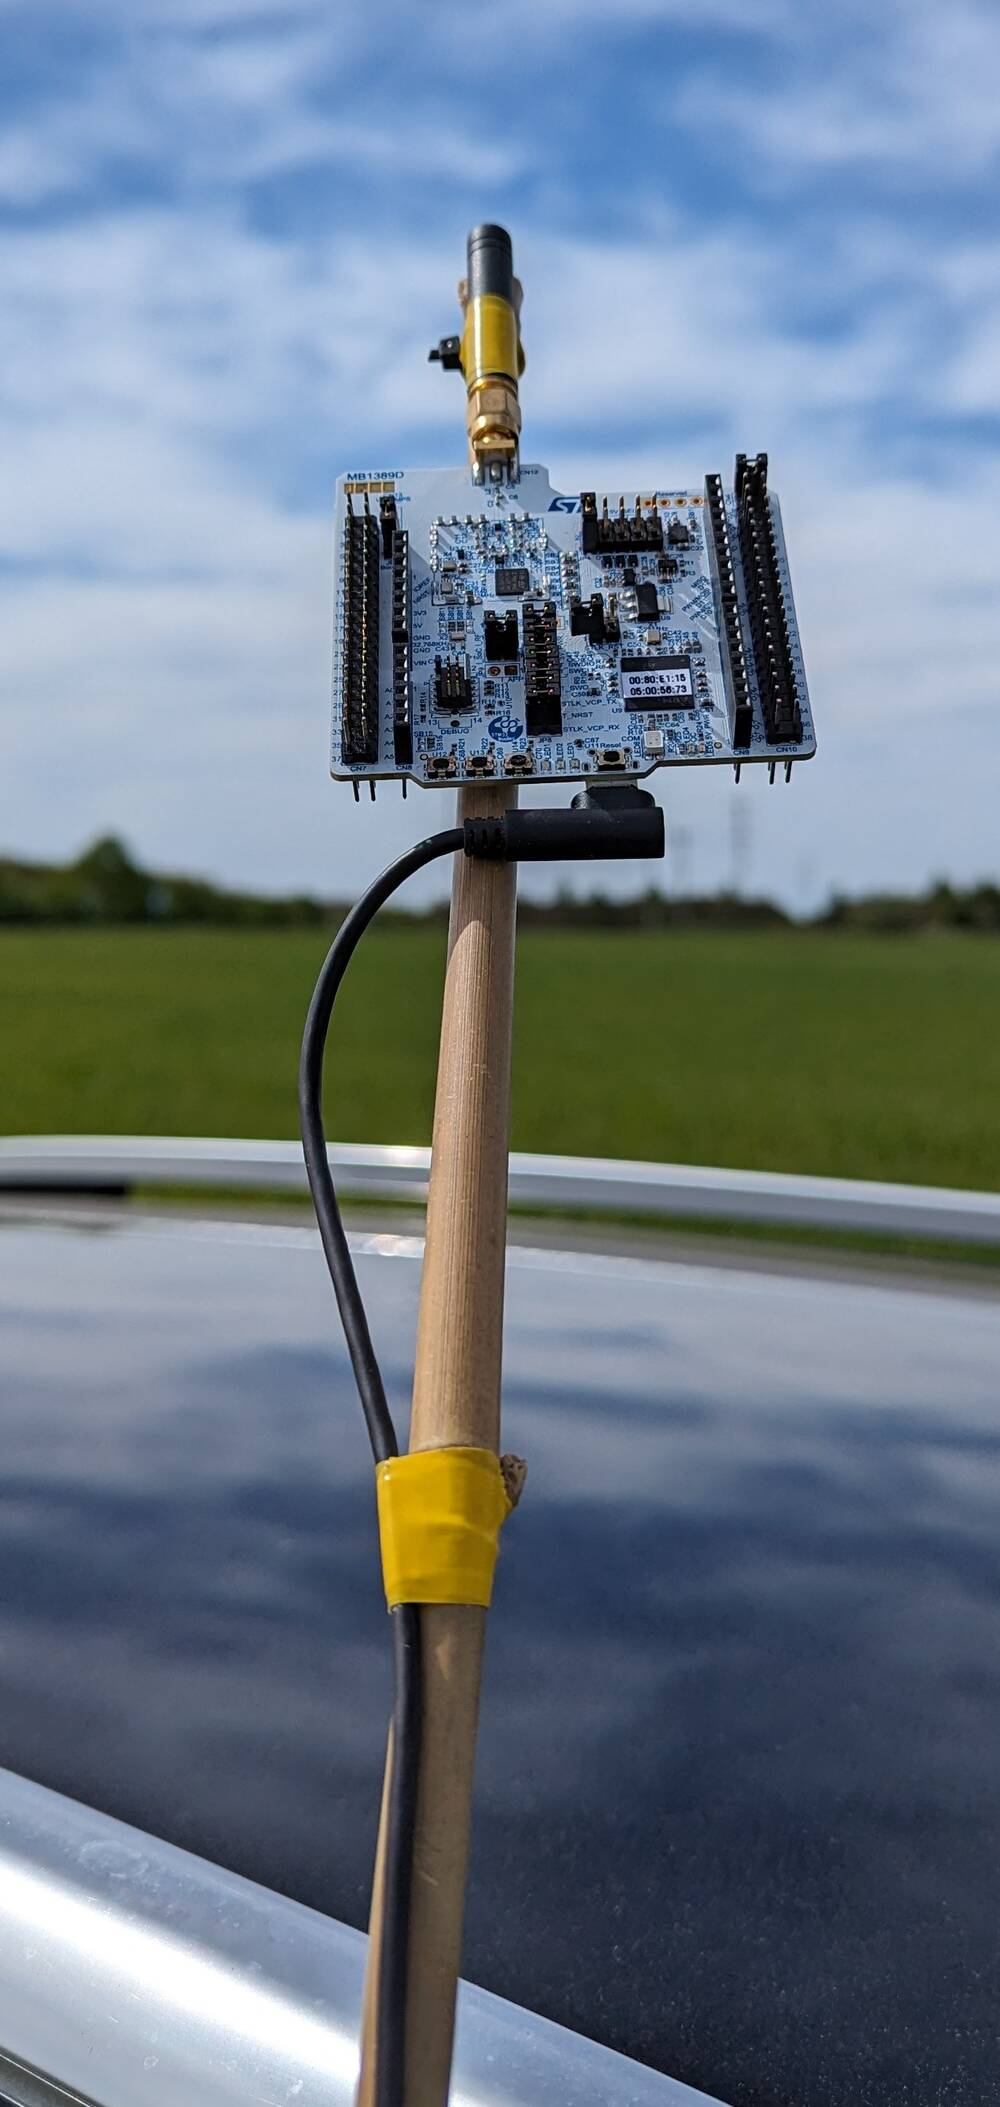
\includegraphics[width=.25\textwidth]{img/range-gateway2.jpg}
    \caption{\label{fig:range-gateway}Close-up of Nucleo attached to the car acting as the Gateway for range testing}
\end{figure}

A location was picked to represent the final use-case, a field with sections of direct line-of-sight and sections obstructed by hills. This place is situated near Průhonice municipality in the Czech Republic. The pole with Nodes attached was installed at \href{https://en.mapy.cz/letecka?q=50.0012006N%2C%2014.5308962E&x=14.5381677&y=50.0011824&z=16}{50.0012006N, 14.5308961E} (WGS84).

A set of measurements was taken through the Gateway at different locations progressing further from the stationary pole with the Nodes attached. These measurements consisted of downloading a random binary 1 KB file to each of the Nodes consecutively. This file was fragmented on the fly by the OTA update protocol to 16 blocks of 64 bytes each.

This means that effectively 16 different measurements of the signal quality were taken at each location for each of the three Nodes. Measurements were recorded by the system in a CSV file containing the time since download started, the amount of packets sent and the last block that was acknowledged - thus a success rate can be calculated. In case the download failed to initiate, nothing gets recorded and that is interpreted as 0\% success rate.

\subsection{Results}

Data is interpreted in the context of the line-of-sight conditions. Graphs show the relief, which was derived from altitude data obtained from the \href{https://api.mapy.cz/v1/elevation}{Seznam.cz elevation API} in 5 m resolution of interpolated coordinates of lines connecting the Nodes and Gateway locations.

\subsubsection{Effect of the Spreading Factor}

\begin{figure}[H]
    \centering
    \subfloat[SF11]{\includesvg[width=\textwidth]{data/range/out/relief-sf11.svg}} \hfil
    \subfloat[SF5]{\includesvg[width=\textwidth]{data/range/out/relief-sf5.svg}}
    \caption{\label{fig:range-relief}Graph of the range test locations, their distance from the pole with Nodes, and the relief in the path of the signal}
\end{figure}

\begin{figure}[H]
    \centering
    \subfloat[SF11]{\includesvg[width=\textwidth]{data/range/out/success-sf11.svg}} \hfil
    \subfloat[SF5]{\includesvg[width=\textwidth]{data/range/out/success-sf5.svg}}
    \caption{\label{fig:range-results}Graph of the range test locations, their distance from the pole with Nodes, and the relief in the path of the signal}
\end{figure}

\begin{figure}[H]
\begin{minipage}[t]{.45\textwidth}
    \vspace{0pt}
    \begin{tabular}{|l|l|l|l|}
\multicolumn{4}{c}{\textbf{SF11}} \\ \hline 
\textbf{Spot} & \textbf{Node 4} & \textbf{Node 3} & \textbf{Node 2} \\ \hline
0 & 100\% & 100\% & 100\% \\ \hline
1 & 100\% & 100\% & 100\% \\ \hline
2 & 100\% & 94\% & 100\% \\ \hline
3 & 100\% & 100\% & 100\% \\ \hline
4 & 100\% & 100\% & 100\% \\ \hline
5 & 100\% & 94\% & 100\% \\ \hline
6 & 100\% & 100\% & 94\% \\ \hline
7 & 100\% & 100\% & 100\% \\ \hline
8 & 94\% & 100\% & 100\% \\ \hline
9 & 100\% & 94\% & 100\% \\ \hline
\end{tabular}

\end{minipage}
\begin{minipage}[t]{.45\textwidth}
    \vspace{0pt}
    %\begin{table}
        \begin{tabular}{|l|l|l|l|}
\multicolumn{4}{c}{\textbf{SF5}} \\ \hline 
\textbf{Spot} & \textbf{Node 4} & \textbf{Node 3} & \textbf{Node 2} \\ \hline
0 & 100\% & 100\% & 100\% \\ \hline
1 & 100\% & 100\% & 100\% \\ \hline
2 & 100\% & 100\% & 100\% \\ \hline
3 & 100\% & 100\% & 100\% \\ \hline
4 & 100\% & 100\% & 100\% \\ \hline
5 & 100\% & 100\% & 100\% \\ \hline
6 & 100\% & 100\% & 100\% \\ \hline
7 & 100\% & 100\% & 0\% \\ \hline
8 & 100\% & 100\% & 0\% \\ \hline
9 & 100\% & 100\% & 0\% \\ \hline
10 & 89\% & 0\% & 0\% \\ \hline
11 & 89\% & 100\% & 0\% \\ \hline
\end{tabular}
    
    %\end{table}
\end{minipage}
\caption{\label{table:range-results}Success rates for each node and location at spreading factors 5 and 11}
\end{figure} 

\subsubsection{Maximum distance}

\begin{figure}[H]
    \centering
    \begin{minipage}[t]{\textwidth}
        \centering
        \begin{tabular}{|l|l|l|l|}
\multicolumn{4}{c}{\textbf{SF11-FAR1}} \\ \hline 
\textbf{Spot} & \textbf{Node 4} & \textbf{Node 3} & \textbf{Node 2} \\ \hline
0 & 100\% & 100\% & 100\% \\ \hline
10 & 100\% & 6\% & 0\% \\ \hline
\end{tabular}

        \vspace{1em}
    \end{minipage}
    \includesvg[width=\textwidth]{data/range/out/relief-sf11-far1-lines.svg}
    \caption{\label{fig:range-relief-far1}Graph of the range test locations, their distance from the pole with Nodes, the relief in the path of the signal and the direct line-of sight lines to each node}
\end{figure}

\begin{figure}[H]
    \centering
    \begin{minipage}[t]{\textwidth}
        \centering
        \begin{tabular}{|l|l|l|l|}
\multicolumn{4}{c}{\textbf{SF11-FAR2}} \\ \hline 
\textbf{Spot} & \textbf{Node 4} & \textbf{Node 3} & \textbf{Node 2} \\ \hline
0 & 100\% & 100\% & 100\% \\ \hline
11 & 100\% & 100\% & 100\% \\ \hline
\end{tabular}

        \vspace{1em}
    \end{minipage}
    \includesvg[width=\textwidth]{data/range/out/relief-sf11-far2-lines.svg}
    \caption{\label{fig:range-relief-far2}Graph of the range test locations, their distance from the pole with Nodes, the relief in the path of the signal and the direct line-of sight lines to each node}
\end{figure}

%\begin{figure}[H]
%\begin{minipage}[t]{.45\textwidth}
%    \vspace{0pt}
%    \begin{tabular}{|l|l|l|l|}
\multicolumn{4}{c}{\textbf{SF11-FAR1}} \\ \hline 
\textbf{Spot} & \textbf{Node 4} & \textbf{Node 3} & \textbf{Node 2} \\ \hline
0 & 100\% & 100\% & 100\% \\ \hline
10 & 100\% & 6\% & 0\% \\ \hline
\end{tabular}

%\end{minipage}
%\begin{minipage}[t]{.45\textwidth}
%    \vspace{0pt}
%    \begin{tabular}{|l|l|l|l|}
\multicolumn{4}{c}{\textbf{SF11-FAR2}} \\ \hline 
\textbf{Spot} & \textbf{Node 4} & \textbf{Node 3} & \textbf{Node 2} \\ \hline
0 & 100\% & 100\% & 100\% \\ \hline
11 & 100\% & 100\% & 100\% \\ \hline
\end{tabular}

%\end{minipage}
%\caption{\label{table:range-results-far}Success rates for each node}
%\end{figure} 

